\chapter{2D Transformation and Alignment}

\noindent
Es fundamental diferenciar las dos operaciones principales de modificación de imágenes en visión por computadora:
\begin{itemize}
    \item \textbf{Image Filtering (Filtrado):} modifica el \textit{rango} (los valores de intensidad/brillo de los píxeles), pero mantiene las posiciones espaciales intactas. Su expresión matemática es 
    $$g(x) = h(f(x))$$
    como por ejemplo Convolución Gaussiana, Sobel.
    \item \textbf{Image Warping (Deformación):} modifica el \textit{dominio} (las posiciones geométricas de los píxeles), mapeando las coordenadas de una imagen a nuevas posiciones espaciales. Su expresión matemática es 
    $$g(x) = f(h(x))$$
    como por ejemplo rotación, distorsión de lente, homografías.
\end{itemize}


\section{Transformaciones 2D}
Para poder representar traslaciones y proyecciones complejas mediante multiplicaciones de matrices compactas, convertimos las coordenadas cartesianas 2D $(x, y)$ en \textbf{Coordenadas Homogéneas} añadiendo un factor de escala $w$ al vector:
$$\begin{bmatrix} x \\ y \end{bmatrix} \Longrightarrow \begin{bmatrix} x_h \\ y_h \\ w \end{bmatrix} = \begin{bmatrix} w \cdot x \\ w \cdot y \\ w \end{bmatrix}$$
Para regresar al plano cartesiano físico, simplemente dividimos las coordenadas escaladas entre el último elemento: $(x, y) = (x_h/w, y_h/w)$. Si $w=1$, las coordenadas corresponden directamente a los píxeles físicos.

\subsection{Tipos de Transformaciones Geométricas 2D}
\noindent
A continuación se detallan las transformaciones geométricas del tema organizadas por sus grados de libertad (DoF) y sus propiedades de invarianza. Todas se expresan como $p' = M \cdot p$:

\subsubsection{1. Traslación (Translation) -- 2 DoF}
\noindent
Desplaza los puntos una distancia fija en el eje $X$ ($t_x$) y en el eje $Y$ ($t_y$):
$$\begin{bmatrix} x' \\ y' \\ 1 \end{bmatrix} = \begin{bmatrix} 1 & 0 & t_x \\ 0 & 1 & t_y \\ 0 & 0 & 1 \end{bmatrix} \begin{bmatrix} x \\ y \\ 1 \end{bmatrix}$$

\subsubsection{2. Rotación (Rotation) -- 1 DoF (3 DoF combinada con traslación)}
\noindent
Gira los puntos un ángulo $\theta$ con respecto al origen de coordenadas de la imagen:
$$\begin{bmatrix} x' \\ y' \\ 1 \end{bmatrix} = \begin{bmatrix} \cos\theta & -\sin\theta & 0 \\ \sin\theta & \cos\theta & 0 \\ 0 & 0 & 1 \end{bmatrix} \begin{bmatrix} x \\ y \\ 1 \end{bmatrix}$$

\subsubsection{3. Escalado (Scaling) -- 2 DoF}
\noindent
Modifica el tamaño de la estructura visual aplicando factores de escala independientes $s_x$ y $s_y$:
$$\begin{bmatrix} x' \\ y' \\ 1 \end{bmatrix} = \begin{bmatrix} s_x & 0 & 0 \\ 0 & s_y & 0 \\ 0 & 0 & 1 \end{bmatrix} \begin{bmatrix} x \\ y \\ 1 \end{bmatrix}$$

\subsubsection{4. Transformación Afín (Affine Transform) -- 6 DoF}
\noindent
Es una transformación lineal general que combina rotación, escalado, traslación y cizalladura (\textit{shear}). Su propiedad fundamental es que \textbf{preserva las líneas paralelas}.
$$\begin{bmatrix} x' \\ y' \\ 1 \end{bmatrix} = \begin{bmatrix} a_1 & a_2 & t_x \\ a_3 & a_4 & t_y \\ 0 & 0 & 1 \end{bmatrix} \begin{bmatrix} x \\ y \\ 1 \end{bmatrix}$$

\begin{definicion}
    Una \tbf{cizalladura (shear)} es una deformación que desplaza los puntos de la imagen en una dirección de forma proporcional a la distancia que tengan respecto a un eje fijo. Los puntos que están en la base (distancia cero) no se mueven nada, y cuanto más subes en altura (coordenada $Y$ más alta), más se desplazan los píxeles hacia un lado (coordenada $X$). \\
\end{definicion}

\noindent
Tenemos dos tipos de cizalladura dependiendo del eje fijo que elijamos:
\begin{itemize}
    \item \tbf{Cizalladura Horizontal (Shear en X):} el eje fijo es el horizontal ($X$), y los píxeles se desplazan horizontalmente según su altura. Su matriz pura es:
    $$\begin{bmatrix} x' \\ y' \\ 1 \end{bmatrix} = \begin{bmatrix} 1 & sh_x & 0 \\ 0 & 1 & 0 \\ 0 & 0 & 1 \end{bmatrix} \begin{bmatrix} x \\ y \\ 1 \end{bmatrix} \implies \begin{cases} x' = x + sh_x \cdot y \\ y' = y \end{cases}$$
    la nueva altura $y'$ se queda exactamente igual. Sin embargo, la nueva posición horizontal $x'$ es la posición original $x$ más un extra que depende de la altura ($y$) multiplicada por el factor de cizalladura $sh_x$.
    
    \item \tbf{Cizalladura Vertical (Shear en Y)}: el eje fijo es el vertical ($Y$), y los píxeles se desplazan verticalmente según su distancia horizontal. Su matriz pura es:
    $$\begin{bmatrix} x' \\ y' \\ 1 \end{bmatrix} = \begin{bmatrix} 1 & 0 & 0 \\ sh_y & 1 & 0 \\ 0 & 0 & 1 \end{bmatrix} \begin{bmatrix} x \\ y \\ 1 \end{bmatrix} \implies \begin{cases} x' = x \\ y' = y + sh_y \cdot x \end{cases}$$
    la nueva posición horizontal $x'$ se queda exactamente igual. Sin embargo, la nueva altura $y'$ es la posición original $y$ más un extra que depende de la distancia horizontal ($x$) multiplicada por el factor de cizalladura $sh_y$.
\end{itemize}

\subsubsection{5. Homografía (Homography / Projective) -- 8 DoF}
\noindent
Es la transformación más general en el plano geométrico. Representa una transformación proyectiva que mapea puntos de un plano físico a otro plano bajo una perspectiva de cámara distinta. \textbf{No preserva el paralelismo}, pero sí preserva la colinealidad (las líneas rectas siguen siendo líneas rectas).
$$\begin{bmatrix} x' \\ y' \\ 1 \end{bmatrix} \sim \begin{bmatrix} h_{11} & h_{12} & h_{13} \\ h_{21} & h_{22} & h_{23} \\ h_{31} & h_{32} & h_{33} \end{bmatrix} \begin{bmatrix} x \\ y \\ 1 \end{bmatrix}$$
Dado que opera bajo un factor de escala global en coordenadas homogéneas, la matriz contiene 9 elementos pero solo **8 grados de libertad independientes** (se suele normalizar fijando $h_{33} = 1$). \\

\noindent
Podemos ver en la Figura \ref{fig:2d_transform} ejemplos de algunas de estas transformaciones.

\begin{figure}
    \centering
    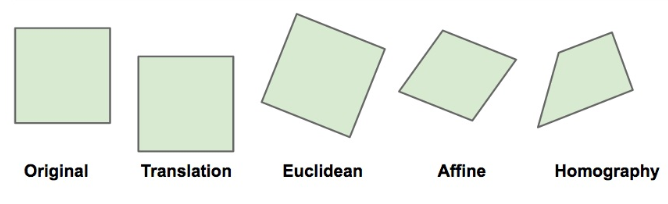
\includegraphics[width=0.8\textwidth]{img/2d_transform.png}
    \caption{Example 2D transformations.}
    \label{fig:2d_transform}
\end{figure}

\section{El Rol Crítico de la Homografía}
La homografía es la herramienta matemática fundamental para dos aplicaciones estrella en computer vision:
\begin{enumerate}
    \item \textbf{Mapeo de Puntos Planares (Planar Mapping):} si los puntos del mundo real yacen sobre una superficie completamente plana (como una pared, el suelo o la portada de un libro), la relación geométrica exacta entre sus posiciones en dos fotos tomadas desde cualquier ángulo de cámara se describe perfectamente mediante una matriz de homografía $H$, por lo que se usa la homografía para enderezar y alinear las imágenes. \\
    
    \noindent
    Aplicaciones como CamScanner (cuando le haces una foto de lado a un folio o a una pizarra y la app la endereza mágicamente como un documento PDF perfecto) usan exactamente este principio de Planar Mapping.
    \item \textbf{Coser Panorámicas (Panorama Stitching):} Cuando creamos una foto panorámica rotando la cámara sobre su propio centro óptico, las imágenes capturadas están relacionadas de forma estricta por una homografía, lo que permite proyectar y ``alinear'' todas las tomas sobre un lienzo virtual común.
\end{enumerate}


\section{Pipeline Completo de Alineamiento de Imágenes}
Para fusionar dos imágenes solapadas y alinearlas de forma automática, el ordenador ejecuta secuencialmente los siguientes pasos:

\begin{enumerate}
    \item \textbf{Detectar Características (Detect Features):} Extraer los puntos clave estables en ambas imágenes independientes utilizando algoritmos como Harris o SIFT, obteniendo las coordenadas $(x, y, \sigma)$.
    \item \textbf{Emparejar Características (Match Features):} Calcular los descriptores vectoriales de apariencia y buscar las correspondencias más sólidas mediante el vecino más cercano (Nearest Neighbor) y filtros de seguridad como el Ratio Test de Lowe.
    \item \textbf{Estimar la Homografía (Estimate Homography):} Filtrar los emparejamientos erróneos (*outliers*) e identificar el modelo matemático mayoritario mediante el algoritmo iterativo \textbf{RANSAC}. Como una homografía tiene 8 DoF y cada punto da 2 ecuaciones, RANSAC toma muestras mínimas de \textbf{$s=4$ parejas de puntos} para calcular matrices candidatas $H$. Al final del consenso, refina la mejor matriz usando todos los \textit{inliers} por mínimos cuadrados.
    \item \textbf{Deformar la Imagen (Warp Image):} Aplicar la matriz de homografía calculada sobre los píxeles de la imagen de origen para proyectarla geométricamente sobre el espacio de coordenadas de la imagen de destino.
\end{enumerate}

\subsection{Mecanismos de Warping: Forward vs. Inverse Mapping}
\noindent
Al ejecutar el último paso de deformación (\textit{warping}), nos enfrentamos a un problema práctico de discretización en la red de píxeles:
\begin{itemize}
    \item \textbf{Forward Mapping:} Toma cada píxel $(x,y)$ de la imagen original y calcula su nueva posición destino $(x', y') = H(x,y)$. \textit{Defecto:} Como las nuevas coordenadas dan números decimales flotantes, al redondearlos a enteros se generan 
    \begin{itemize}
        \item \tbf{Huecos vacíos:} habrá píxeles en la imagen de destino donde ningún píxel de origen cayó al redondear. Esos píxeles se quedarán negros, creando una desagradable ``red de puntos negros'' o agujeros en tu imagen deformada.
        \item \tbf{Solapamientos}: dos píxeles de origen distintos podrían terminar redondeando a la misma coordenada de destino, peleándose por ver quién pinta encima.
    \end{itemize}    

    \item \textbf{Inverse Mapping (Mapeo Inverso):} Soluciona el problema recorriendo cada píxel $(x', y')$ de la pantalla de destino vacía. Aplica la homografía inversa para calcular de qué píxel exacto de la imagen original debió venir: $(x, y) = H^{-1}(x', y')$. Luego, lee el color en esa coordenada de origen. \\
    
    \noindent
    Dado que $H^{-1}(x', y')$ devolverá valores decimales flotantes (por ejemplo, venir del píxel origen $x=45.3, y=20.1$), se aplican técnicas de \tbf{interpolación} para estimar el color real combinando los píxeles vecinos:
    \begin{itemize}
        \item \tbf{Nearest Neighbor Interpolation:} toma el color del píxel entero más cercano. Es rápido pero genera bordes pixelados (``serruchado'').
        \item \tbf{Bilinear Interpolation:} realiza un promedio ponderado lineal combinando los 4 píxeles que rodean la coordenada decimal. Genera transiciones suaves y texturas continuas de alta calidad.
    \end{itemize}
\end{itemize}

\section{Pipeline de Transformación de Coordenadas de Cámara}
Para entender de dónde surgen estas transformaciones espaciales en las fotos, debemos trazar el camino físico que recorre un punto del universo tridimensional hasta plasmarse en la pantalla digital del ordenador:

$$\mathbf{P_{world}} \xrightarrow{\quad [R \mid t] \quad} \mathbf{P_{camera}} \xrightarrow{\quad K \quad} \mathbf{p_{image}}$$

\begin{enumerate}
    \item \textbf{Punto en el Mundo ($\mathbf{P_{world}}$):} coordenadas 3D reales del objeto medidas respecto a un origen global arbitrario del universo $(X_w, Y_w, Z_w)$.
    \item \textbf{Coordenadas de Cámara ($\mathbf{P_{camera}}$):} se transforma la posición del punto del mundo al sistema de coordenadas local del ojo de la cámara aplicando una rotación $R$ y una traslación $t$ (parámetros extrínsecos de la cámara). El punto pasa a medirse con respecto al centro óptico de la lente.
    \item \textbf{Coordenadas de Imagen ($\mathbf{p_{image}}$):} el punto 3D de la cámara se proyecta sobre el plano del sensor fotosensible mediante la matriz de calibración intrínseca $K$, la cual tiene en cuenta la distancia focal ($f$) y el centro del plano del sensor ($c_x, c_y$). El resultado es la coordenada discreta de píxeles $(x, y)$ que procesamos en nuestro código.
\end{enumerate}

\noindent
Todos estos conceptos de distancia focal, centro del plano del sensor y parámetros extrísicos e intrínsicos de la cámara se estudian en profundidad en el tema de calibración de cámaras (Tema 14), pero es importante entender que las transformaciones 2D que aplicamos a las imágenes son una consecuencia directa de cómo la geometría del mundo real se proyecta a través de la lente y se captura en el sensor digital.

